%\chapter{State of the art}
\label{chap:chapter2}

\section[Stack Overflow]{\glsentrylong{so} (\glsentryshort{so})}
\label{sec:stackoverflow}

\subsection[Stack Overflows design]{\glsentrylong{so}s (\glsentryshort{so}) Design}
\label{sec:stackoverflow_design}
The following lists the factors that were used when designing \gls{so} (based on \textcite[p.~6-7]{M.Sewak2010} and \textcite[p.~805]{Treude2011}):
\begin{enumerate}
	\item Votes: Questions and answers which are considered good (or bad) by the community can be given a score. 
	This gives a filtering mechanisms, which allows users to ignore answers that are bad or wrong. 
	Furthermore, answers are sorted by votes, and you can also sort questions on \gls{so} by vote score 
	(see Figure \ref{fig:question_list_acc_answ}). 
	\item Accepted answer: If the user asking a question gets an answer that they find satisfactory, they can select it as the "accepted answer". 
	This answer will be the first displayed of the answers, and is also viewable when searching for questions 
	(see Figure \ref{fig:question_list_acc_answ} and \ref{fig:so_question_example}).
	\item Tags: Each question is associated with a tag\footnote{
		A full list can be seen here: \url{http://stackoverflow.com/tags/}
	}, which can be a topic, a programming language, a methodology, etc.
	\item Badges: Similar to achievements in games, Badges are used to reward the user for their participation.
	\item Reputation and Bounty: Currency system for user participation. 
	E.g. voting for questions, getting your answer selected as the accepted one, etc.
	Bounty is a trade, where if your question goes unanswered for too long, you offer up parts of your reputation to receive an answer.
	\item Data dump: Available data dump containing all content available within the \gls{se} community \cite{StackExchange2016}. 
	You can either download single files, or everything by using a Torrent client.
	\item Pre-Search: Encouraging users to check that their question is not already posted by presenting a search bar when asking a new question. 
	\item URL keywords and Google: The questions title is included in the URL, allowing it to be processed by search engines. 
	In addition, Google uses their crawlers every 10 second to have the latest updates from \glossary{so} in their search engine \cite{Gobry2011}.
	\item Critical mass: Before Atwood and Spoolsky launched \gls{so}, they invited developers and programmers to participate to have some domain experts available. 
\end{enumerate}

\clearpage
% figure showing questions, where one question has an accepted answer
\begin{figure}[ht]
	\centering
	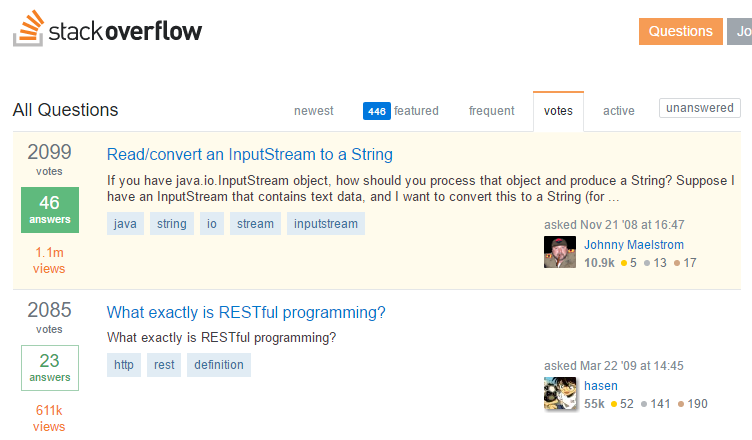
\includegraphics[width=0.5\textwidth]{question_list_acc_answ}
	\caption{List of questions, where one can see those with an accepted answers are marked with a green background.}
	\label{fig:question_list_acc_answ}
\end{figure}


% figure showing page with question and answer
\begin{figure}[ht]
	\centering
	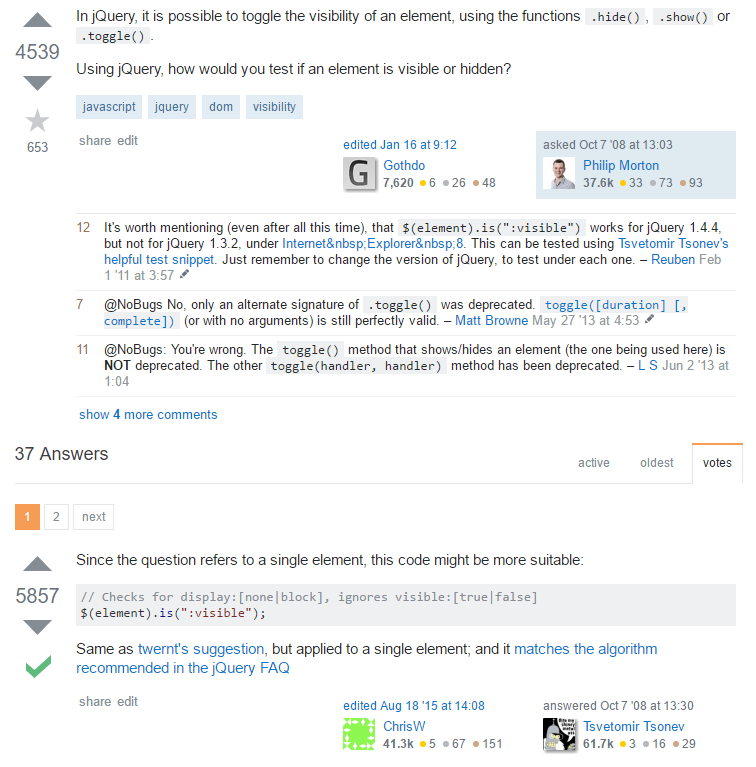
\includegraphics[width=0.5\textwidth]{so_question_example}
	\caption[Example of a question on Stack Overflow]{Example of a question on Stack Overflow\footnotemark}
	\label{fig:so_question_example}
\end{figure}
\footnotetext{Source: \url{http://stackoverflow.com/questions/178325/checking-if-an-element-is-hidden}}

\subsection[Stack Overflow and Gamification]{\glsentrylong{so} (\glsentryshort{so}) and Gamification}
\label{sec:stackoverflow_gamification}
\textcite{Deterding2011} defines Gamification as "the use of game design elements in non-game contexts", and is the definition this section will be based on. 
Several papers make notes of the pedagogical and educational aspect of \gls{so} \cite{Nasehi2012, Posnett2012, Yang2014}, and \cite{Nasehi2012, Yang2014} use the term gamification in their paper.
One of the founders, Jeff Atwood said in an interview that he wanted users to not just give good answers, but also trick them into improving their communication skills \cite{Posnett2012}\footnote{
	From this interview: \\ 
	\url{http://www.wired.com/2012/07/stackoverflow-jeff-atwood/2012}.
	}.
In the course IMT4007 Serious Games Simon McCallum and Marius Nowostawski, presented their game GoRad, which was based on us students reading articles and posting questions which were voted on. 
The \gls{so} system awards users based their activity by using votes, reputation and badges \cite{M.Sewak2010, Movshovitz-Attias2013, Treude2011, StackOverflow.com2016, StackOverflow.com2016d}.
\vspace{0.5em}\newline
If you look at \gls{so} as a game, users could be represented as the four player types presented in \cite[p.~3]{Maan2013}: Achievers, Explorers, Socializers and Killers. 
These player types can be used as a representation\footnote{	
	\textcite{Yang2014} characterised users as "Sparrows" and "Owls", where sparrows answers question for reputation and owls answers the difficult ones (domain experts).  \\
	\textcite[p.~2]{Ahmed2015} defined users as "lurkers, help-seekers (askers) and givers (responders)".	
	} for the various users of \gls{so}. 
Achievers are there for the reputation and badges, socializers are to interact, discuss and share knowledge. 
Explorers might find joy in looking at various topics, or searching for unanswered questions.
The only exception would be the "Killer" type. 
\textcite[p.~3]{Maan2013} defines Killers as those "\ldots who always want to create trouble/problems for other participants" (although this would be more fitting for the term "Griefer"). 
In an online \gls{qa} system (or Internet in general), these are what are commonly referred to as "Trolls" \cite{Fosdick2012, Atwood2015}. 
However, due to the system used in \gls{so}, Trolls would not be able to survive, simply because the reputation controls what you have access to \cite{StackOverflow.com2016g}. 
If you down-vote a post, you lose reputation. 
If your post gets down-voted, you also lose reputation. 
Users who are not willing to follow the guidelines can be locked out of \gls{so} \cite{Atwood2009}.
However, today there is a lot of blogs complaining about the current structure of \gls{so}, who claims that a lot of the moderators are
trolls\footnote{\url{https://www.reddit.com/r/programming/comments/3cafkp/is_stack_overflow_overrun_by_trolls/}. \\	
	\url{https://medium.com/@johnslegers/the-decline-of-stack-overflow-7cb69faa575d} \\ 
	Last accessed 23.05.2016. 
}.

\subsection[Stack Overflow and reputation]{\glsentrylong{so} (\glsentryshort{so}) and reputation}
\label{sec:research_on_so}

Many \gls{qa} sites includes domain experts to ensure some quality is upheld, and uses voting and reputation as a quality measurement \cite{Anderson2012}.
Furthermore, questions topics, page views and votes can be used by search engines as a ranking mechanism, and it helps users to find the answers they are looking for. 
\textcite{Anderson2012} identifies two principles for the answer process. 
This process starts with the question being filtered down through the users, starting with domain experts. 
If the domain experts does not answer, it goes further down the chain, until it in the end either gets an answer, or is not answered at all.
Both \textcite{Anderson2012} and \textcite{Treude2011} defines an unanswered question to be a question where no accepted answer is chosen\footnote{
	However, they do not take into considerations users who find a solution on their own, or simply forget or neglect to mark a an answer as accepted.
}. 
The second principle is that a questions activity level does not just indicate the interest for the question, but could also be an indicator for quality 
(because a question can have multiple answers). 
\vspace{0.5em}\newline
Since users can only gain 200 reputation points daily, the only way to earn more is by having your answer marked as accepted or through bounties \cite{StackOverflow.com2016d}.
\textcite{Movshovitz-Attias2013} found that users earn more reputation by providing good answers rather than good 
questions\footnote{
	However, as stated in \textcite[p.~3]{Movshovitz-Attias2013}, the reputation system was changed at one point. 
	Originally, up-votes on questions and answers gave users a +10, but this was later changed into up-votes on questions only giving +5. 
}.
Most questions was asked by the users with a low reputation, but on average users with high reputation asked more questions. 
This indicates that reputation could be used as a measurement for expertise. 
\textcite{Ahmed2015} also found that there was a correlation between amount of answers given and the users reputation.
\vspace{0.5em}\newline
\textcite{Yang2014} found that the activity level of a user is not equal to knowledge, and divided users into two groups; "Sparrows" and "Owls".
The sparrows are the basic users who earns reputation and badges by answering the easy questions, and has a greater interest in the gamification element. 
They found that the sparrows usually has a low average score and targets questions that are easy, or non-relevant. 
Nonetheless, they are still important since they are able to provide quick feedback.
As for the owls, they are considered to be the domain experts.
The owls earn reputation by asking more advanced questions, providing better answers (i.e. getting their answer accepted) and answering popular and difficult\footnote{
	Popularity was measured based on page views and the time between a question was posted until an answer was selected as accepted.
	The popularity can also therefore be seen as a measurement for difficulty.
	The longer it takes to answer, the more difficult the question is~\cite[p.~273]{Yang2014}.
} questions.
\vspace{0.5em}\newline
\textcite{Posnett2012} views \gls{se} and \gls{so} as a learning community, since users help each gain new knowledge, and motivates learning.
They wanted to see if the quality of the users answers improved over time. 
By constructing a posting history for each user, they found that the overall answer score decreased, and that the answer quality was static.
\vspace{0.5em}\newline
\textcite{Nasehi2012} did a qualitative analysis of code examples posted on \gls{so}. 
Their focus was on questions related to Java programming, with the requirements that the question should at least have a score of +4 and the answer +7. 
In addition, a code example should be included (by checking for <code> in the post).
They found that the code explanation was just as important as the code examples (but you are still restricted to the quality of that example).
For the code to be considered good, they listed the following attributes: 
\begin{enumerate}
	\item Concise code: Code samples should not be too long. 
	They should be simple, and only focus on the parts that are relevant to the topic.
	Additional or non-relevant parts should instead be documented by using descriptive comments.
	\item Question context: 
	If the code is not working properly, suggestions for improvement should be added. 
	One could also explain best practices and suggestions for improved readability.
	This will also have a pedagogical benefit, since the user asking the questions will learn to write better code.
	\item Highlighting important elements: 
	"Straight to the point", clearing up misunderstandings, pointing to relevant resources, etc.
	\item Step-by-step solution: 
	Splitting code into chunks, and explaining each chunk and its functionality.
	Comparison of languages; e.g. "How can I do X in C\#, when I'm used to Java?"
	\item Providing links to extra resources: 
	Answers can be kept short by adding links to external resources, but a short summary should still be added.
\end{enumerate}


\section{Asking questions}
\label{sec:asking_questions}

\subsection{What is the definition of a question?}
\label{sec:question_definition}
The context of a question varies within the setting it is used. 
A question can be broad, where multiple answers can all be correct, or they can be factual, having only one right answer. 
When you are asking someone a question, you ask because you want to either find a solution to a problem, or learn something new. 
In the context of learning, questions are used for evaluating the students knowledge, or help them learn something new \textcite{Nielsen2008}.
\vspace{0.5em}\newline
When doing research, you need research questions and hypotheses to decide what the goal of your research is. 
What questions are you trying to find an answer to, and what does that answer tell you?
\textcite{Slowiaczek1992} defines asking a question as information selection and the answer(s) to a question as information usage. 
If you are working with statistical data, and you just post the numbers, this will not inform anyone. 
You need to explain what the numbers mean, and how you got them.
The quality of an answer is also restricted to the quality of the question you ask. 
One can therefore assume that if you ask a good question, you increase the chance of getting a good answer \cite{Slowiaczek1992}. 

\subsection[Question classification]{\glsentrylong{qc} (\glsentryshort{qc})}
\label{sec:question_classification}
\gls{qc} is the process of categorizing a question into a class or category based on its structure, usually to decide what the expected answer type is \cite{Li, Loni2011, Lopez2011}. 
To classify a question, it is important to select only those features that helps you identify the class it belongs to.
To get a classification results, you use what is known as a classifier. 
The quality of a classifier can be measured by its accuracy and precision (see Equation \ref{eq:accuracy} and \ref{eq:precision}; taken from \cite[p.~13]{Li}).

\begin{equation}\label{eq:accuracy}
Accuracy = \frac{\#~of~correct~predictions}{\#~of~predictions}
\end{equation}

\begin{equation}\label{eq:precision}
Precison[c] = \frac{\#~of~correct~predictions~of~class~c}{\#~of~prediction~of~class~c}
\end{equation}

\paragraph{WH-words}
\label{sec:wh_words}
WH-words are mostly found in factoid questions \cite{Lopez2011}. 
\textcite{Huang2008} listed eight different WH-words: What, which, when, where, who, how, why, and rest (rest being the type does not belong to any of the previous type). 
\textcite{Letovsky1987} also listed "Whether" and "Discrepancy"\footnote{
	"Questions that reflect confusion over a perceived inconsistency." \cite[p.~5]{Letovsky1987}
}.
However, not all are equally easy to use for classification, because even if the questions ask for the same answer, wording and syntactic structures can make it difficult to classify.
Question containing words like "What", "Why", "How" and "Which", can be harder to classify due to the lack of limitation in regards to answer types\footnote{
	An answer type (or named entity) is the expected type of the answer to a given question (e.g. a Location, Organization, Person, Date, etc) \cite{Heie2012, Lopez2011, Sasaki2005, Yen2013}. 
} \cite{Huang2008, Lopez2011}.


\paragraph[Bag-of-words and N-grams]{\glsentrylong{bow} (\glsentryshort{bow}) and N-grams}
\label{sec:bow}
N-gram is a model that is used for splitting text into either characters (character model) or word frequencies (word model). 
The \gls{bow} model (or unigram) only looks at singular words, ignoring the order and relies only on the frequency for each word \cite{Manning2008, Russell2013}. 
Bi-grams takes dual values, tri-gram takes three, etc.
\vspace{0.5em}\newline
One problem with N-grams is that the dimension of the feature space is equal to the amount of words in the vocabulary \cite{Russell2013, Loni2011}
When using categorization, there can be issues with mapping new words that does not exist in the vocabulary \cite{Yen2013}.
The impact of N-gram is also related to the size of the text being analysed. 
\textcite{Zhang2003} found that there was not a big difference when using between bag-of-ngrams (all continuous word sequences in the question) and \gls{bow} as features.


\paragraph{Word mapping and processing: Case-sensitivity, Stemming, Stop words and Tokenization}
\label{sec:word_mapping_processing}
To reduce the number of words used, there are more steps that can be taken. 
By removing the case-sensitivity, all words will be equal (e.g. is the word 'Hello' equal to the word 'hello'?).
\cite{Huang2008} includes case-sensitivity under a definition called word shape, consisting of five elements: upper case, all lower case, mixed case, all digits, and other.
\vspace{0.5em}\newline
Semantics can be used for word filtering, e.g. removal of duplicate words or words with same meaning. 
WordNet has a built in function called synsets() which removes synonyms (words having the same meaning). 
You can also look for hypernyms (words belonging to a category with a parent-child relationship) or use stemming.
Stemming reduces the word to its base-form, e.g. crying would be converted into the word cry.
Word separation is also possible through tokenization, which splits the text into an array based on a set delimiter.
There is also usage of stop words for removal of frequently used words in a given language.
\vspace{0.5em}\newline
%Stop words \cite{Manevitz2002, Wang2013, Zhang2003, Kaestner2013, Joachims1998}
Grammatical properties can be extracted by using \gls{pos}, e.g. by using \gls{nltk}\footnote{
	\gls{nltk} includes in their \gls{pos} tagger the following grammatical properties:
	Adjective, adposition, adverb, conjuction, determiner, article, noun, numeral, particle, pronoun, verb, 
	punctuation mark and others	 \cite[See Section 2.3]{StevenBird2015}.
}, which can be helpful in reducing ambiguities \cite{Bloehdorn2004}.
\textcite{Li} uses the word head chunks to identify what the question is asking for when multiple types are introduced (avoid ambiguity). 
The same concept is used in \cite{Huang2008} and \cite{Loni2011}, but there it is referred to as headwords.

\subsection{Text classification}
\label{sec:text_classification}
The goal of text classification (or text categorization) is to be able to process multiple documents or large amounts of text into categories. 
It shares similarities with question classification, although an obvious difference would be the size of the text that is processed. 
Some examples are spam filtering \cite{Russell2013, Kaestner2013}, to identify languages, or filing documents based on content \cite{Kaestner2013}.
Documents can belong in more then category, and since categories can overlap they must be treated as a binary classification problem \cite{Joachims1998} .
Text classification starts with retrieval of the documents, usually by using \gls{ir} methods, and then transforming the text into features for the classification. 
When you have a large amount of text, you can easily get a feature space that is very high dimensional, and that is why feature selection is important. 
Feature selection is the selection of features (or attributes) that are important for the classification. 
E.g. if you were classifying documents based on colour description, then hypernyms for colour would be an important feature.


\subsection[Question-Answering]{\glsentrylong{qa} (\glsentryshort{qa})}
\label{sec:question_answering}
\gls{qa} is mostly used as a method for finding the answer to a question from an unknown amount of documents.
When using a search engine, one can accept that there are several results that are listed because at least one of the search terms exists. 
However, when using a \gls{qa} system, users wants the answer straight away instead of having to read through several documents. 
In addition, \gls{qa} sites allows users to search for questions in the same way they would ask another human (natural language\footnote{
	However, there is a problem with linguistics in natural language systems \cite{Lopez2011}.
	}), 
and there are also different types of \gls{qa} sites.
Domain specific \gls{qa} focuses on a specific topic (e.g. \gls{so}) and open domain where everything goes. 
\gls{qa} sites can also function as an archive or a knowledge base, since all the posts are available even years after they were posted.
\vspace{0.5em}\newline
\textcite{Yen2013} found that it was more efficient searching for answers in a small dataset, then the document as a whole. 
By using a passage retriever, the documents were split into paragraphs and ranked by using evaluation metrics. 
\textcite{Isozaki2005} could not use TF-IDF based paragraph retrieval, because the paragraphs were too short to cover all query terms. 
If the terms that were used were too short or too long, the passage scores would not reflect the density distribution. 
\textcite{Xu2012} built an online \gls{qa} system for tourism, which consisted of question analysis, information retrieval and answer extraction.
Since rule-based approach requires expert knowledge, creating features that are domain specific can improve accuracy (what they called "domain term concept hierarchy").
To validate the classification, they tested the results by using 5-fold cross-validation.
\vspace{0.5em}\newline
\textcite{Li} used semantics to categorize questions based on the possible semantic answer type. 
One issue with questions are that since they can be very short, they contain little text. 
However, the lack of long text improves both the accuracy and analysis. 
\vspace{0.5em}\newline
\textcite{Zhang2003} says that \gls{qc} is important, and simply looking for WH-words is not enough. 
By using WH-words, headwords, WordNet semantics, N-grams and word shapes as features, and a linear \gls{svm} and Maximum Entropy model, 
they reached an 89.2\% and 89.0\% over a standard benchmark dataset. 
They also experimented with four other algorithms, Nearest Neighbours (simplified version of k-NN),  Naive Bayes and Decision Tree and Sparse Network of Winnows (SNoW).
However, these were outperformed by the \gls{svm}.


\section[SVM]{\glsentrylong{svm} (\glsentryshort{svm})}
\label{sec:svm}

\gls{svm}s are good for solving regression and classification problems, and attempts to solve a linearly separable problem by using hyperplanes \cite{Duda2001, Kononenko2007, Russell2013}.
It is usually used for binary classifications, where classes are represented as either +1 or -1 \cite{Manning2008, Russell2013}. 
The hyperplane is the plane which separates the two classes: 
% hyperplane equation
\begin{equation}\label{eq:hyperplane}
\vec{w}^{T}\vec{x} = \textit{-b} 
\end{equation}
where \textit{b} is the intercept term and $\vec{w}$ is the weight vector (or decision hyperplane normal vector).
The data set can be represented as $\mathbb{D} = \{(\vec{x}_{i}, y_{i})\}$ where $\vec{x}_{i}$ is a data point, and $ y_{i}$ is its belonging class label.
The linear classifier is represented in Equation \ref{eq:linear_classifier}  \cite[p.~295-296]{Manning2008}. 
% linear classifier
\begin{equation}\label{eq:linear_classifier}
f(\vec{x}) = sign(\vec{w}^{T}\vec{x} + b)
\end{equation}
% space
In addition to using a hyperplane, the \gls{svm} has an additional separation known as support vectors. 
Support vectors are the training points closest to the margin (the margin is the distance from the hyperplane) \cite{Duda2001, Manning2008}.
Which then gives that the optimal hyperplane is the furthest from the support vectors \cite{Kononenko2007}.
% space
\gls{svm} has four different kernels, but a limitation is that there is no way to select the best kernel function. 
Therefore, \gls{svm} often uses hyper-parameters and select the classifier based on the best results \cite{Theodoridis2009}.
Equation \ref{eq:kernel_polynomial} - \ref{eq:kernel_sigmoid} shows the kernel functions (K) for polynomial, radial basis function (RBF) and sigmoid (taken from \cite[p.~273]{Kononenko2007}). \\
% polynomial kernel
Polynomial - for a given polynomial degree \textit{d}, the following is used:
\begin{equation}\label{eq:kernel_polynomial}
K (\textbf{x}_{j}, \textbf{x}) = [(\textbf{x}  \cdot \textbf{x}_{j}) + 1]^{d}
\end{equation}
% rbf kernel
Radial - for a given $\gamma$ value, the following is used:
\begin{equation}\label{eq:kernel_rbf}
K (\textbf{x}_{j}, \textbf{x}) = e^{-\gamma|\textbf{x}-\textbf{x}_{j}|^{2}}
\end{equation}
% sigmoid kernel
Sigmoid - for a given sigmoid function S, we get a kernel function of parameters \textit{v} and \textit{c}: 
\begin{equation}\label{eq:kernel_sigmoid}
K (\textbf{x}_{j}, \textbf{x}) = S(\textit{v}(\textbf{x}  \cdot \textbf{x}_{j}) + c)
\end{equation}

For text classification, in most cases it will be non-linearly separable. 
One can therefore allow the \gls{svm} to do some mistakes.
However, there is a cost for misclassifications, represented by what is called a slack variable $\xi_{i}$.
If $\xi_{i}$ is set (not zero), then the vector can miss the margin requirement at the cost of $\xi_{i}$.
Equations are shown in Equation \ref{eq:slack_variable1} - \ref{eq:slack_variable3} (taken from \cite[p.~301]{Manning2008}). \\
Find
% slack variable optimization - 1
\begin{equation}\label{eq:slack_variable1}
\vec{w}, b~and~\xi_{i} \geq 0
\end{equation}
% slack variable optimization - 2
so that we can minimize the optimization problem
\begin{equation}\label{eq:slack_variable2}
\frac{1}{2}\vec{w}^{T}\vec{w}~+~C\sum_{i}\xi_{i}
\end{equation}
% slack variable optimization - 3
and for all
\begin{equation}\label{eq:slack_variable3}
\{(x_{i}, y_{i})\},~y_{i}(\vec{w}^{T}\vec{x}~+~b) \geq 1 - \xi_{i}
\end{equation}
However, this gives a trade-off between the size of the margin and how much the data points can be adjusted. 
To avoid overfitting, the parameter C is used for regularization, where the size of C decides how much flexibility you get from the slack variable \cite{Manning2008}.
\gls{svm} neither suffer from the Curse of dimensionality, because the computational complexity is independent of the kernels dimensional space~\cite{Theodoridis2009}.


% SHOULD THIS BE USED?
%\gls{svm} uses the maximum margin solution, which is based on computational learning theory\footnote{	
%	Computational learning theory is an attempt to understand how large a data set needs to be in order to give good generalization \cite[p.~344]{Bishop2006}.
%} \cite{Bishop2006, Joachims1998}.
%% keep this sentence; its properly re-written
%For \gls{qc} a question is usually represented as a vector space model, where each vector contains the words from the question \cite{Loni2011}.

\textcite{Joachims1998} found that \gls{svm} consistently achieved good performance during text categorization. 
Since \gls{svm} could generalize in high dimensional feature space, the need for feature selection was removed, and \gls{svm} was also robust. 
Since \gls{svm} does not require parameter tuning, they could find good parameter settings automatically. 
\textcite{Loni2011} found that \gls{svm} are successful on high dimensional data when it is sparse, but they still suffer from redundant features. 

\begin{comment}
% Re-write and use what ever fits
\gls{svm}s
are very successful on high dimensional data since they are
timely efficient especially when the feature vectors are sparse,
but they still suffer from the redundant features.
\gls{svm} is a linear discriminant model which tries to find a
hyperplane with maximum margin for separating the classes.
They are fast classifiers for high dimensional data [13]. To
be able to linearly separate data, the feature space usually is
mapped to a higher dimensional space. The mapping is done
with a so-called kernel function. The most widely used kernel
in question classification is the linear kernel. 
\cite{Loni2011}


\gls{svm} is based on the Structural Risk Minimization principle from computational learning theory. 
The idea of structural risk minimization is to find a hypothesis h for which we can guarantee the lowest true error.  
The true error of h is the probability that h will make an error on an unseen and randomly selected test example. 
An upper bound can be used to connect the true error of a hypothesis h with the error of h on the training set and the complexity of H (measured by VC-Dimension), the hypothesis space containing h. 
\gls{svm}s find the hypothesis h which (approximately) minimizes this bound on the true error by effectively and efficiently controlling the VC-Dimension of H.
One remarkable property of \gls{svm}s is that their ability to learn can be independent of the dimensionality of the feature space. 
\gls{svm}s measure the complexity of hypotheses based on the margin with which they separate the data, not the number of features. 
This means that we can generalize even in the presence of very many features, if our data is separable with a wide margin using functions from the hypothesis space. 
The same margin argument also suggest a heuristic for selecting good parameter settings for the learner (like the kernel width in all RBF network). 
The best parameter setting is the one which produces the hypothesis with the lowest VC-Dimension.
This allows fully automatic parameter tuning without expensive cross-validation. \\
Theoretical analysis concludes that \gls{svm}s acknowledge the particular properties of text: 
\begin{itemize}
\item high dimensional feature spaces, 
\item few irrelevant features (dense concept vector), 
\item sparse instance vectors.
\end{itemize}
Experimental results show that \gls{svm}s consistently achieve good performance on text categorization tasks, outperforming existing methods substantially and significantly. 
With their ability to generalize well in high dimensional feature spaces, \gls{svm}s eliminate the need for feature selection, making the application of text categorization considerably easier.
Another advantage of \gls{svm}s over the conventional methods is their robustness. 
\gls{svm}s show good performance in all experiments, avoiding catastrophic failure, as observed with the conventional methods on some tasks. 
Furthermore, \gls{svm}s do not require any parameter tuning, since they can find good parameter settings automatically. 
All this makes \gls{svm}s a very promising and easy-to-use method for learning text classifiers from examples.
\cite{Joachims1998}
\end{comment}

